%!TEX root = structure.tex

\section{Introduction}
Ceci est l'introduction à mon projet sur les pavages de Truchet.

\section{Réflexions diverses}

Je dois penser à mes systèmes de Truchet comme à des espaces mathématiques dans lesquels je peux me déplacer, un peu comme l'ensemble de Mandelbrot est un espace mathématique. Je peux créer des \textit{ensembles de Truchet} que mon système pourra visualiser à n'importe quelles valeurs.

Idéalement, il me faudrait pouvoir définir mes ensembles de Truchet ainsi :
Un groupe de 4 permutations : A, C, B, A, miroité horizontalement avec A, B, C, A, et miroité verticalement avec X, X, X, X.

Essentiellement, je dois pouvoir définir un bloc, de telle largeur et telle hauteur, et ensuite, définir ses répétitions et, optionnellement, ses symétries.

\begin{lstlisting}
var block = {
    lines : [ABBACDAB, CDDBDADD],
    horizontalSymmetry: true,
    verticalSymmetry: false,
    diagonalSymmetry: false
};
\end{lstlisting}

La combinaison de la symétrie horizontale et de la symétrie verticale crée automatiquement une symétrie diagonale.

\section{Transitions animées entre les positions des tuiles}
Il me faut absolument créer des transitions animées entre les diverses positions que les tuiles de Truchet peuvent prendre. Il pourrait y avoir des transitions dans le sens des aiguilles d'une montre et des transitions dans le sens inverse. L'usage de ces 2 sens pourrait créer des effets variés, et même être combinés (mais je ne sais pas exatement comment, pour l'instant).

J'ai même l'impression que tout est peut-être là. Tout le charme du film pourrait être dans ces transitions-là. Parce que des animations de pavages de Truchet sans transitions, comme je l'ai expérimenté hier soir (20 mars 2017), ça fait très froid. Ça fait peu musical, également.

\section{Les différents morceaux}

\subsection{Une feuille d'instructions}

Il me faut une feuille d'instructions, qui est essentiellement un espace mathématique. Une feuille d'instruction contient : une largeur et une hauteur en nombres entiers, une booléenne \textit{horizontalSymmetry} et une booléenne \textit{verticalSymmetry}. Et finalement, une feuille d'instruction contient soit des données statiques qui remplissent sa largeur et sa hauteur, soit un lien vers une autre feuille d'instruction, avec une valeur \textit{offset} qui sera un vecteur en nombre entier.

Donc, ça donne ça
\begin{lstlisting}
//First type of block, with static data.
var blockOne = {
    type : "static",
    size : {x: 8, y: 4},
    data : ["ABBACDAB", "CDDBDADD", "CDABCDAB", "DADDDADD"],
    horizontalSymmetry: true,
    verticalSymmetry: false
};

//Second type of block, with a reference to another block.
var blockTwo = {
    type : "dynamic",
    size : {x: 8, y: 2},
    data : {
        ref: blockOne,
        offset: {x: 50, y: 50}
    },
    horizontalSymmetry: true,
    verticalSymmetry: true
};
\end{lstlisting}
\newpage
Et si je créais un bloc ainsi? Est-ce qu'un bloc devrait avoir son propre array \textit{fullSpace}? Dans tous les cas, lorsque je me déplace à l'intérieur de l'espace mathématique d'un bloc, je ne devrais pas avoir à recalculer chaque fois chacune des cellules de cet espace mathématique. Il faut que ce grand array \textit{fullSpace} existe quelque part. Et comme il est, conceptuellement, une propriété du bloc, il devrait peut-être devenir factuellement une propriété du bloc. 

Le seul problème que j'envisage avec ce système, c'est le cas des blocs dynamiques. Les blocs dynamiques créent forcément des valeurs \textit{fullSpace} différentes. Il faudrait peut-être simplement que les blocs dynamiques aient une méthode \textit{reCalculateFullSpace}. Étrangement, cette fonction se retrouverait à scruter dans la valeur \textit{fullSpace} d'un autre bloc. Ainsi, animer un bloc dynamique, ça voudrait dire changer sa valeur \textit{offset} dans le temps, ce qui ferait que ce bloc scruterait un autre bloc à une position spatiale changeante.

\begin{lstlisting}
var Block = function(block) {
    this.type = block.type;
    this.size = block.size;
    this.data = block.data;
    this.horizontalSymmetry = block.horizontalSymmetry;
    this.verticalSymmetry = block.verticalSymmetry;
    this.fullSpace = this.makeLargeSpace(block)
};

Block.prototype.makeLargeSpace = function(block) {
    var largeArray = [];
    //Make copies to take care of symmetries,
    //to end up with blocks that can be copied simply without symmetry.

    //And then, make a large amount of copies.
    //Return the large array.
};

var blockOne = new Block({
    type : "dynamic",
    size : {x: 8, y: 2},
    data : {
        ref: blockOne,
        offset: {x: 50, y: 50}
    },
    horizontalSymmetry: true,
    verticalSymmetry: true,
    maxSize : {x: 500, y:700}
});



\end{lstlisting}
\subsection{Une fonction chercheuse}

Il me faut une fonction chercheuse, qui posera ses questions aux feuilles d'instructions.

\begin{lstlisting}
// Voici comment je dois pouvoir appeler la fonction chercheuse.
sheetSearcher({
    startX: 50,
    startY: 50,
    ref: blockOne
});

//Mais comment puis-la définir?
function sheetSearcher(instructions) {
    var truchetValue;
    if (instructions.startX == 0 && instructions.starty == 0) {
        truchetValue = instructions.ref.data[0][0];
    }
    return truchetValue;
}
\end{lstlisting}
La fonction chercheuse reçoit la question suivante : À l'endroit x = 50, y = 50, quelle est la valeur Truchet (A, B, C ou D) de \textit{blockOne}? Elle commence à répondre à cette question en posant la question à \textit{blockOne} : à la valeur x = 0, y = 0, quelle est ta valeur Truchet? Et ensuite, si j'augmente le x de 1, quelle est ta valeur Truchet? La fonction chercheuse commence à trouver la valeur x = 50, y = 0, et ensuite, elle se déplace sur l'axe Y, toujours en posant une question à \textit{blockOne} pour chaque déplacement unitaire. Les booléennes de \textit{blockOne} sont évidemment déterminantes du comportement de la fonction chercheuse. Elle se sert de ces booléennes pour se déplacer à l'intérieur de l'espace mathématique créé par la feuille d'instructions.

Une bien meilleure idée pour l'algorithme de la fonction chercheuse : Elle va se servir des instructions de la feuille d'instruction pour créer un énorme pavage (en copiant les données et créant un énorme array), et ensuite elle se servira de ce pavage pour créer le pavage final. Elle ne génère ainsi les données qu'une seule fois.

\subsection{Une fonction tilingFiller}
Il me faut une fonction qui remplisse un pavage \textit{final}. Cette fonction utilise la fonction chercheuse.
\begin{lstlisting}
// Voici comment je dois pouvoir appeler la fonction remplissante.
var myTiling = tilingFiller({
    size: {width: 32, height: 18},
    ref: blockOne,
    offset: {x: 10, y: 10}
});

// Et la définition de cette fonction.
function tilingFiller(instructions) {
    var tiling = [];
    for (var x = 0; x < instruction.size.width; x += 1) {
        for (var y = 0; y < instruction.size.height; y += 1) {
            var truchetValue = sheetSeeker({
                startX: instructions.offset.x,
                startY: instructions.offset.y,
                ref: instructions.ref
            });
            //Important de réviser ceci avant l'usage :
            tiling[x + y * instructions.size.width] = truchetValue;
        }
    }
    return tiling;
}

//Version diaboliquement plus simple de tilingFiller() :

//Ici je crée quelque chose de statique... je crée un pavage qui sera appliqué. 
//Mais d'où vient cet appel à la fonction \textit{tilingFiller()}?
var myTiling = tilingFiller({
    inputBlock: blockOne,
    offset: {x: 70, y: 70},
    outputSize : {width: 32, height:18}
});

function tilingFiller(instructions) {
    var block = instructions.inputBlock;
    var offset = instructions.offset;
    var size = instructions.outputSize;
    var tiling = [];
    for (var x = 0; x < size.width; x += 1) {
        for (var y = 0; y < size.height; y += 1) {
            tiling[x + y * size.width] = block.fullSpace[(offset.x + x) + ((offset.y + y) * size.width)];
        }
    }
    return tiling;
}
\end{lstlisting}
\subsection{Des zones alpha animables pour les pavages}

Il me faut une façon de définir essentiellement la zone alpha et la position d'un pavage, qui pourront être animées par le système d'animation.

\newpage
\subsection{La x-sheet}

Et comment vais-je gérer la x-sheet?

\begin{lstlisting}
var xSheet = {
    ailleurs: {
        d: 40,
        f: function(sum) {
            tiling00302.update();
        }
    },
    ailleurs2: {
        d: 200,
        f: function(sum) {
            var rN = getSum(xSheet, xSheet.ailleurs);
            var coFade = cosineFade(sum, 400);
            tiling00515.mixSame(rN, tiling00302, rN, coFade);
        }
    }
};
\end{lstlisting}

\subsection{Transitions entre les diverses positions de Truchet}

Je dois pouvoir avoir un système qui reçoit ces instructions :

\begin{lstlisting}
showTile({
    permutationOne: "A",
    permutationTwo: "C",
    lerpValue: 0.25,
    position: {x: 5, y: 10},
    tileWidth: tileWidth,
    light: color(255,255,150),
    dark: color(50,50,0)
});
\end{lstlisting}

\newpage
\section{Vers de nouvelles animations}
Maintenant que j'ai passé quelques semaines à observer les premiers travaux que j'ai effectués avec les pavages de Truchet, je suis obligé de m'avouer que mes animations ne sont tout simplement pas très intéressantes. Elles sont mathématiquement intéressantes, mais visuellement, je ne suis pas charmé. J'ai eu plusieurs nouvelles idées, cependant. Je crois que la façon la plus efficace de créer des scènes animées avec des pavages de Truchet sera tout simplement de faire changer les pavés d'un coup, sans transition. Les \textit{transitions} seront plutôt définies par l'ordre dans lequel les pavés sont remplacés.

Je peux imaginer l'image finale du film comme une matrice à deux dimensions, dont chaque position contient une lettre (A, B, C, D, E, F), et des informations de couleurs (une couleur pour la partie claire, une couleur pour la partie foncée.

Ensuite, je peux imaginer qu'un pavage (appelé en ce moment un \textit{block}, mais je n'aime pas tellement ce nom) puisse avoir différentes \textit{méthodes de population d'un pavage}, c'est-à-dire, différents algorithmes pour remplir la matrice finale du film avec ses propres données.

Je pourrais même créer une machine à créer automatiquement des pavages et ensuite, à lancer les différentes méthodes de population de la matrice, et voir devant moi un film d'animation infini.

Et évidemment, il me faudrait une xSheet pour planifier le lancement de ces méthodes de population. Le hic, c'est qu'il me faudrait créer un système qui me permettrait de connaître le travail accompli par chaque méthode de population de chaque pavage à n'importe quelle valeur de la xSheet.

Donc, toutes mes méthodes de population doivent recevoir une valeur \textit{t} et répondre avec une matrice. C'est la seule façon de fonctionner.

Et la xSheet, en lançant les méthodes de population de plusieurs pavages en même temps, donnera toujours la même matrice finale.

\begin{lstlisting}
var xSheet = {
    introduction: {
        d: 450,
        f: function(sum) {
            // var rN = getSum(xSheet, xSheet.grotte);
            tiling03.populate(sum);
            tiling15.populate(sum);
        }
    }
};
\end{lstlisting}
\newpage
\subsection{Les méthodes \textit{populate()}}

Essentiellement, la méthode \textit{populate()} devra, à tous les coups, activer son système comme si \textit{t = 0} et avancer jusqu'à ce que \textit{t} égale la vraie valeur \textit{t} demandée en argument. Et \textit{t} ne peut pas être négatif. 
Donc, $(t \in \mathbb{Z}) \land (t \geq 0)$.

Comme je n'ai affaires qu'à des matrices finales à 576 valeurs, ces calculs seront minimes.

\subsubsection{Définition des méthodes \textit{populate()}}
Les méthodes \textit{populate()} seront nombreuses et pourraient être elles-mêmes générées de manière algorithmique. Elles devront évidemment être définies à l'extérieur des objets de type \textit{Block}, donc en fait il ne s'agit pas de méthodes mais simplement de fonctions.

Ce devrait être la xSheet qui permet de lancer telle méthode de population sur tel Block.
\begin{lstlisting}
    //la xSheet lance la méthode populate() de l'objet redTiling, 
    //en lui envoyant une fonction de population choisie, ici diagonalFury.
    //diagonalFury reçoit l'argument qui deviendra t à l'intérieur de la fonction.

    //diagonalFury() renvoit une matrice dont les éléments sont true ou false.
    //populate() se sert de cette matrice pour remplir chaque case true avec
    //une valeur A, B, C, D, E, ou F, et deux valeurs de couleur.
    redTiling.populate(diagonalFury(sum));
\end{lstlisting}

En fait, lors de sa création, une fonction de population pourrait très bien générer une liste statique de matrices, et la méthode \textit{populate()} d'un Block pourrait simplement se référer à l'item \textit{t} de cette liste. Je vois certains problèmes avec cette méthode, principalement le fait qu'une méthode de population pourrait très bien avoir un temps d'application infini.

Ceci m'amène à une autre idée : Le but d'une fonction de population pourrait ne pas être simplement de passer d'aucune case habitée à toutes les cases habitées. Une fonction pourrait simplement définir un ensemble de cases habitées selon une valeur \textit{t}, et $t = n$ pourrait très bien contenir un plus grand nombre de cases habitées que $t = n+1$. Donc, des incréments de valeur $t$ pourrait enlever des membres de la population.

\newpage
\section{Génération de pavages colorés et aléatoires}

Avant de me lancer dans les animations avec mes fonctions de population, je dois m'occuper de ce qui est la prochaine étape naturelle : expérimenter avec les pavages colorés et avec la génération de pavages aléatoires.

La génération de pavages aléatoires se fait en plusieurs étapes :

\begin{lstlisting}
//we establish the width of the repeated block. All blocks are square.
var blockWidth = 4;
var blockData = [];
//Then, it is a combination of randomized tile decisions and applications of symmetry.
//for (var i = 0; i < blockWidth; i++) {
//    getRandomTile();
//}
var builtBlocks = 0;
while (builtBlocks < blockWidth) {
    for (var i = 0; i <= builtBlocks; i++){
        blockData[builtBlocks] = blockData[builtBlocks] + getRandomTile();
    }
    builtBlocks++;
}

function getRandomTile() {
    var tiles = ["A", "B", "C", "D", "E", "F"];
    var tile = tiles[round(random(0, 5))];
    return tile;
}

function getSymmetricalTile(tile, type) {
    if (tile == "E" || tile == "F") {
        return tile;
    }
    if (tile == "A" && type = "horizontal") {
        return "D";
    }
    if (tile == "A" && type = "vertical") {
        return "B";
    }
    if (tile == "A" && type = "oblique") {
        return "C";
    }
    if (tile == "B" && type = "horizontal") {
        return "C";
    }
    if (tile == "B" && type = "vertical") {
        return "A";
    }
    if (tile == "B" && type = "oblique") {
        return "D";
    }
    if (tile == "C" && type = "horizontal") {
        return "B";
    }
    if (tile == "C" && type = "vertical") {
        return "D";
    }
    if (tile == "C" && type = "oblique") {
        return "A";
    }
    if (tile == "D" && type = "horizontal") {
        return "A";
    }
    if (tile == "D" && type = "vertical") {
        return "C";
    }
    if (tile == "D" && type = "oblique") {
        return "B";
    }
}

\end{lstlisting}

\section{Couleurs}

Les couleurs d'une tuile doivent être définies ainsi : 
\begin{lstlisting}
var colorTile = {
    l: {
        r: 255,
        g: 150,
        b: 150
    },
    d: {
        r: 55,
        g: 25,
        b: 50
    }
};
\end{lstlisting}

\newpage
\section{Motifs créés par diverses erreurs}

J'ai créé plusieurs images très intéressantes qui sont basées sur des erreurs dans mon algorithme, et je dois comprendre ces erreurs afin de pouvoir bien saisir la génèse de ces images.

\subsection{Mauvais algorithme d'affichage des pavés}
En premier lieu, j'ai créé un nouvel algorithme d'affichage pour mes pavés, qui utilise une énorme quantité de petits points au lieu d'une simple forme géométrique (un carré ou un triangle isocèle rectangle). Mais en créant cet algorithme, j'ai dû me tromper quelque part parce que mes pavages sont devenus complètement défectueux.

Voici à quoi ressemble mon algorithme pour l'instant : 
\begin{lstlisting}
function showNumeralDotted(position, x, y, tW, light, dark) {
    var s = 1;
    // fill(light.r, light.g, light.b, 50);
    for (var i = 0; i < 4500 * 4; i++) {
        var randomDotX = x + random(0, tW);
        var randomDotY = y + random(0, tW);
        // ellipse(randomDotX, randomDotY, 1);
        boxOfDots.push({
            x: randomDotX,
            y: randomDotY,
            s: s,
            r: red(light),
            g: green(light),
            b: blue(light)
        });
    }
    // fill(dark.r, dark.g, dark.b, 50);
    for (var i = 0; i < 4500 * 4; i++) {
        var randomDotX = x + random(0, tW);
        var randomDotY = y + random(0, tW);
        // if (randomDotY < -randomDotX + x + y + tW) {
        //     ellipse(randomDotX, randomDotY, 1);
        // }
        switch (position) {
            case "A":
                if (randomDotY < randomDotX) {
                    showDot(randomDotX, randomDotY, s);
                }
                break;
            case "B":
                if (randomDotY > -randomDotX + x + y + tW) {
                    showDot(randomDotX, randomDotY, s);
                }
                break;
            case "C":
                if (randomDotY > randomDotX) {
                    showDot(randomDotX, randomDotY, s);
                }
                break;
            case "D":
                if (randomDotY < -randomDotX + x + y + width) {
                    showDot(randomDotX, randomDotY, s);
                }
                break;
            case "E":
                break;
            case "F":
                showDot(randomDotX, randomDotY, s);
                break;
            default:
                console.log("Error, not tile type read.");
        }
    }

    function showDot(x, y, s) {
        // ellipse(x, y, s);
        boxOfDots.push({
            x: x * 1.01,
            y: y * 1.01,
            s: s,
            r: red(dark),
            g: green(dark),
            b: blue(dark)
        });
    }
}
\end{lstlisting}

\begin{figure}[h]
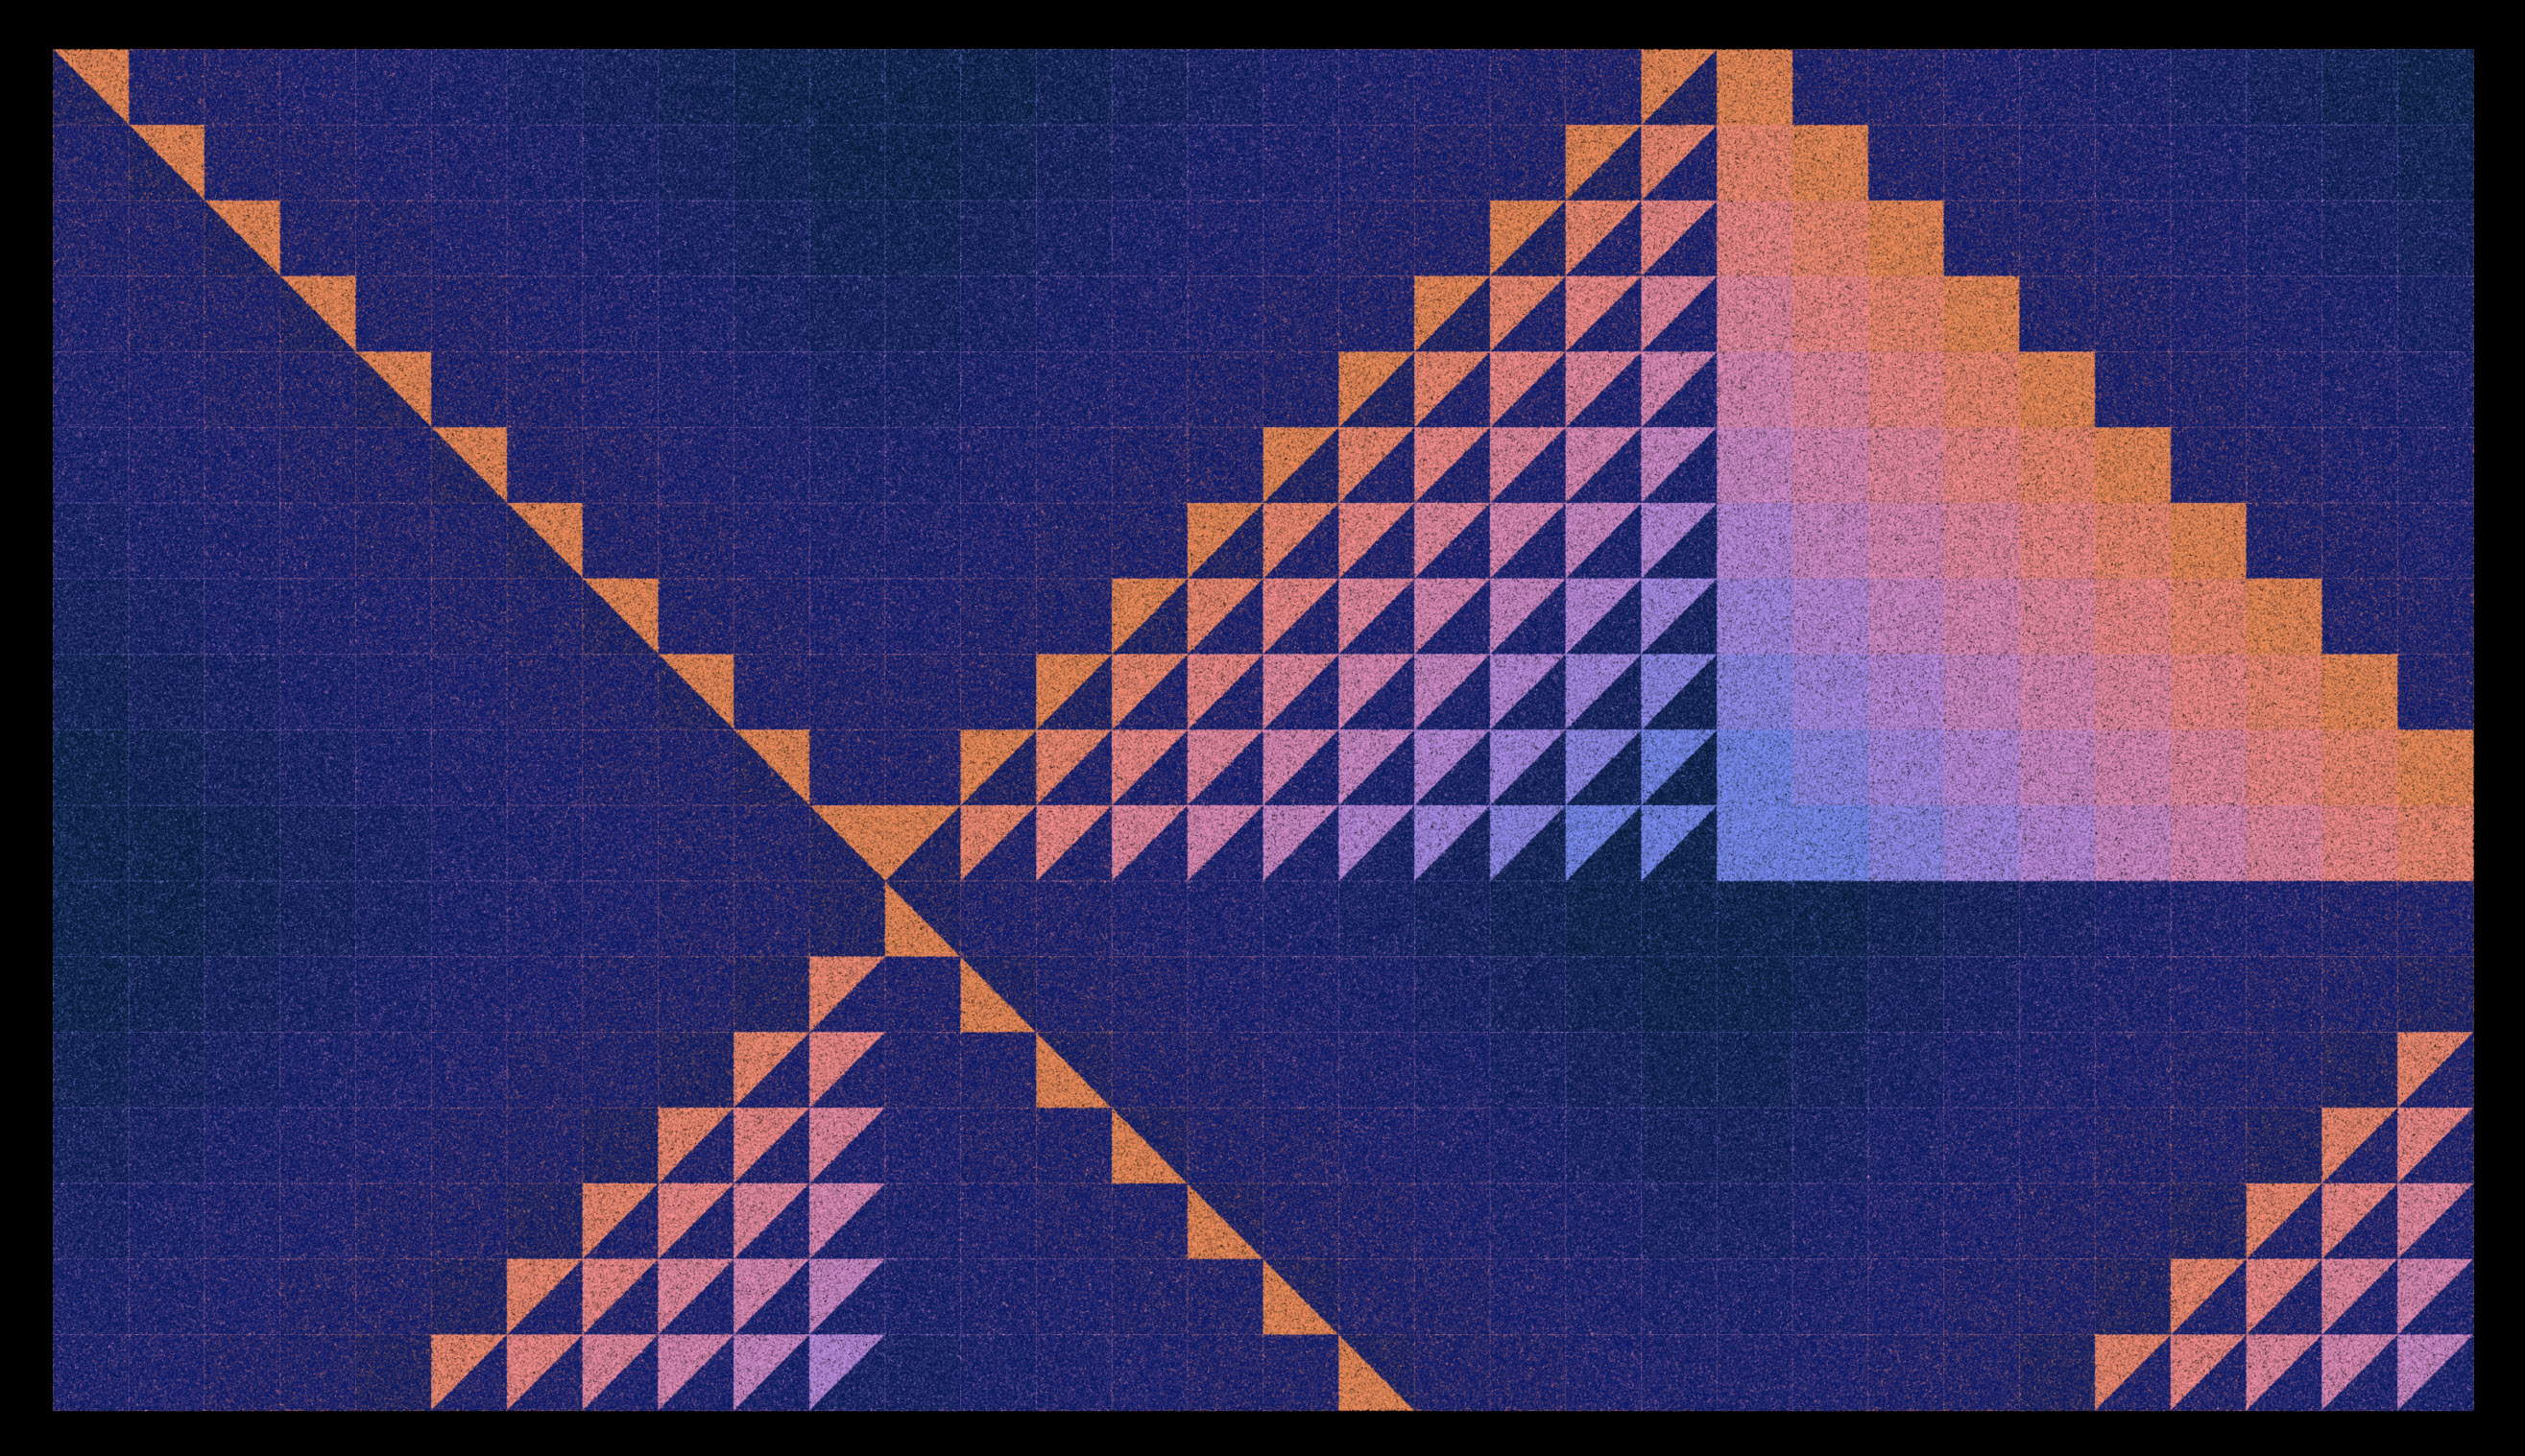
\includegraphics[width=1\textwidth]{images/pavage002.jpg}
\caption{Pavage avec les gouttières normales}
\label{normalgutters}
\end{figure}

\subsection{Largeur des gouttières entre les pavés}
Une erreur spécifique introduite par cet algorithme l'a été après coup. J'ai voulu élargir la zone sur laquelle les points de chaque tuile sont \textit{imprimés} afin de faire disparaître les toutes petites gouttières qu'il y avait entre les tuiles (visibles dans la figure \ref{normalgutters}). Mais ma méthode est défectueuse. J'ai multiplié par 1,01 les valeurs $x$ et $y$ conservées à la toute fin pour \textit{l'impression}. En faisant cela, j'ai plutôt décalé chacune des tuiles d'un certain pourcentage de leurs valeurs $x$ et $y$. Et une tuile décalée se retrouve forcément à se faire \textit{imprimer dessus} par une autre tuile.

\begin{lstlisting}
function showDot(x, y, s) {
    // When the x and y values are multiplied like below, it introduces a gradual shift of the tiles.
    boxOfDots.push({
        x: x * 1.01,
        y: y * 1.01,
        s: s,
        r: red(dark),
        g: green(dark),
        b: blue(dark)
    });
}
\end{lstlisting}

\begin{figure}[h]
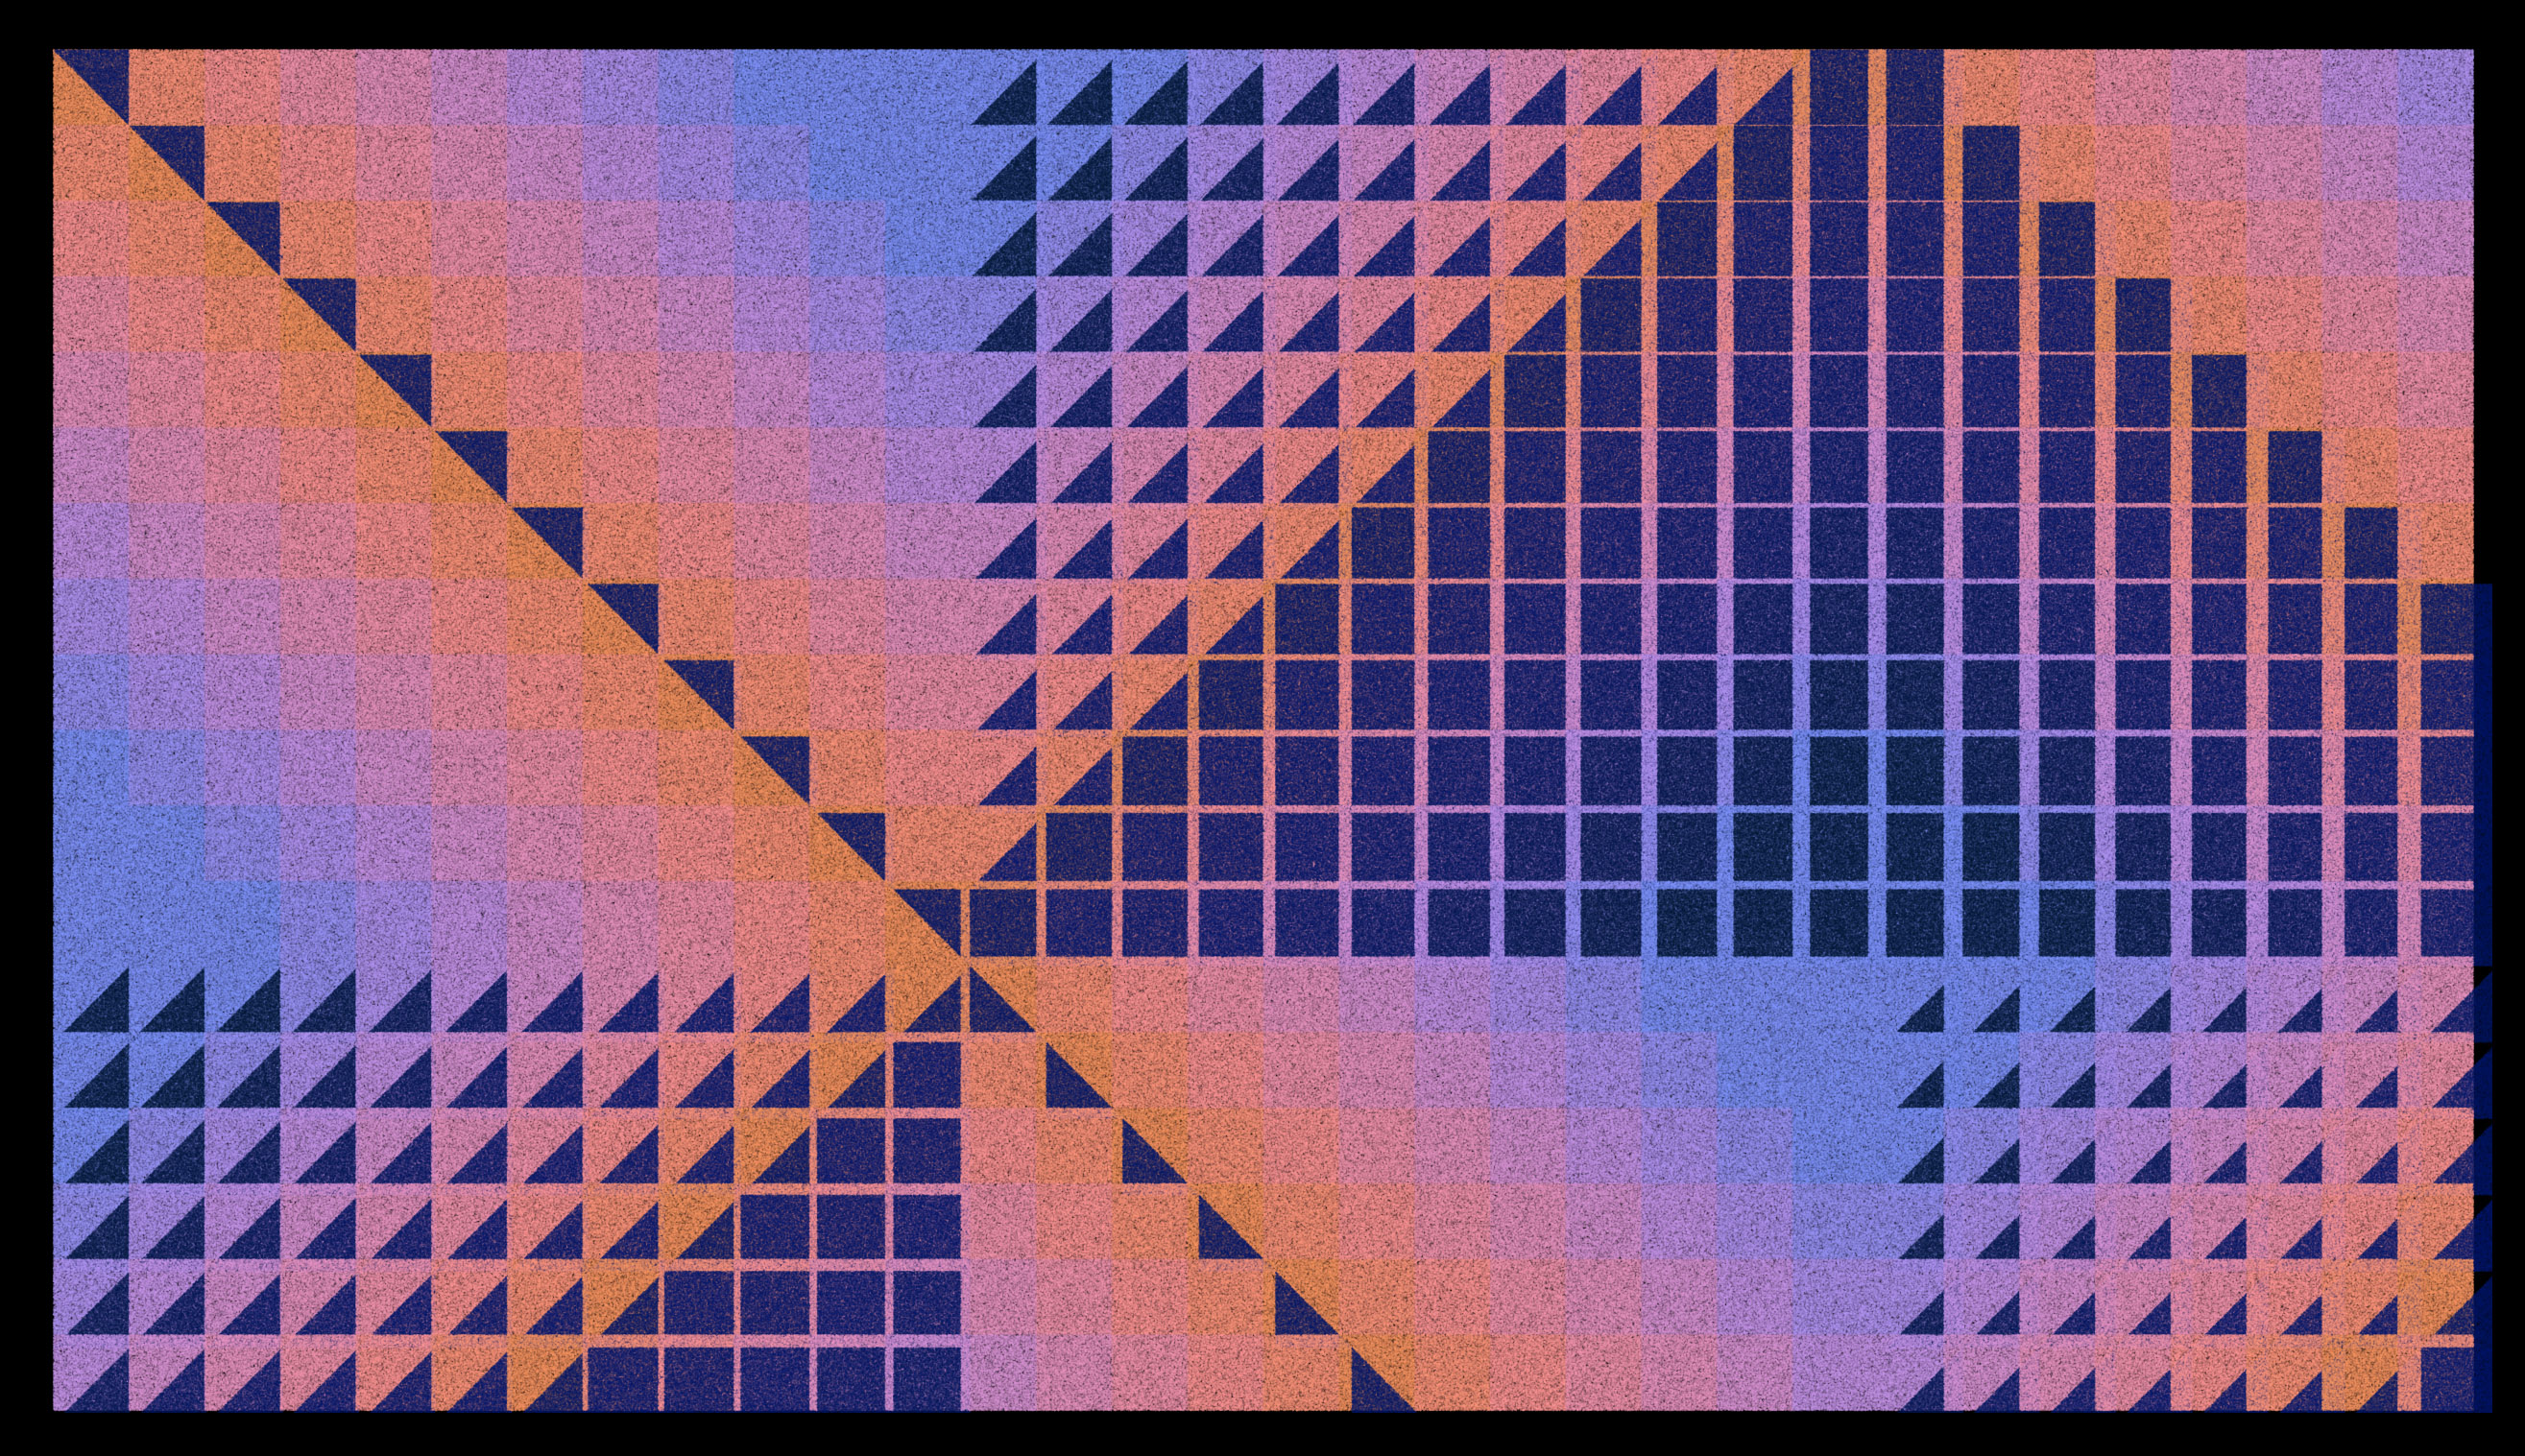
\includegraphics[width=1\textwidth]{images/pavage001.jpg}
\caption{Avec de plus larges gouttières}
\label{largegutters}
\end{figure}
Donc, ce résultat inattendu est en fait très intéressant et pourrait être utilisé encore. La valeur de cette multiplication pourrait être définie de façon algorithmique et produire une variété d'effets animés, par exemple.

\newpage
\section{Couleurs algorithmiques à conserver}
Au travers de tous ces problèmes, j'ai créé trois algorithmes de coloration qui sont très intéressants et que je dois bien documenter afin de ne pas perdre. Voici le troisième : 

\subsection{Second algorithme de coloration}
Le second algorithme est le bleu et orange, celui qui me fait penser à l'heure magique. C'est mon préféré pour l'instant. C'est avec lui qu'ont été créées les images \ref{normalgutters} et \ref{largegutters}. Voici l'algorithme : 
\begin{lstlisting}
//These are the bits used at the creation or shifting of a seed, to asign tile colors.
var red = maps(Math.sin(frames / 5), -1, 1, 0, 255);
var green = maps(Math.cos(frames / 5), -1, 1, 0, 255);
var blue = maps(Math.sin(frames / 5), -1, 1, 0, 105);
colorData[builtBlocks][0] = new ColorTile([red, 150, green, 0, 20, blue]);
\end{lstlisting}

\subsection{Troisième algorithme de coloration}
Celui-ci c'est le vert, rose et brun. Il est utilisé dans l'image \ref{thirdcoloralgorithm}. J'aime particulièrement comment le brun vient jouer avec les autres couleurs.
\begin{lstlisting}
//These are the bits used at the creation or shifting of a seed, to asign tile colors.
var red = maps(Math.sin(frames / 5), -1, 1, 0, 255);
var green = maps(Math.cos(frames / 5), -1, 1, 0, 255);
var blue = maps(Math.sin(frames / 5), -1, 1, 0, 105);
colorData[builtBlocks][0] = new ColorTile([green, red, 150, blue, 20, 0]);
\end{lstlisting}

\begin{figure}[h]
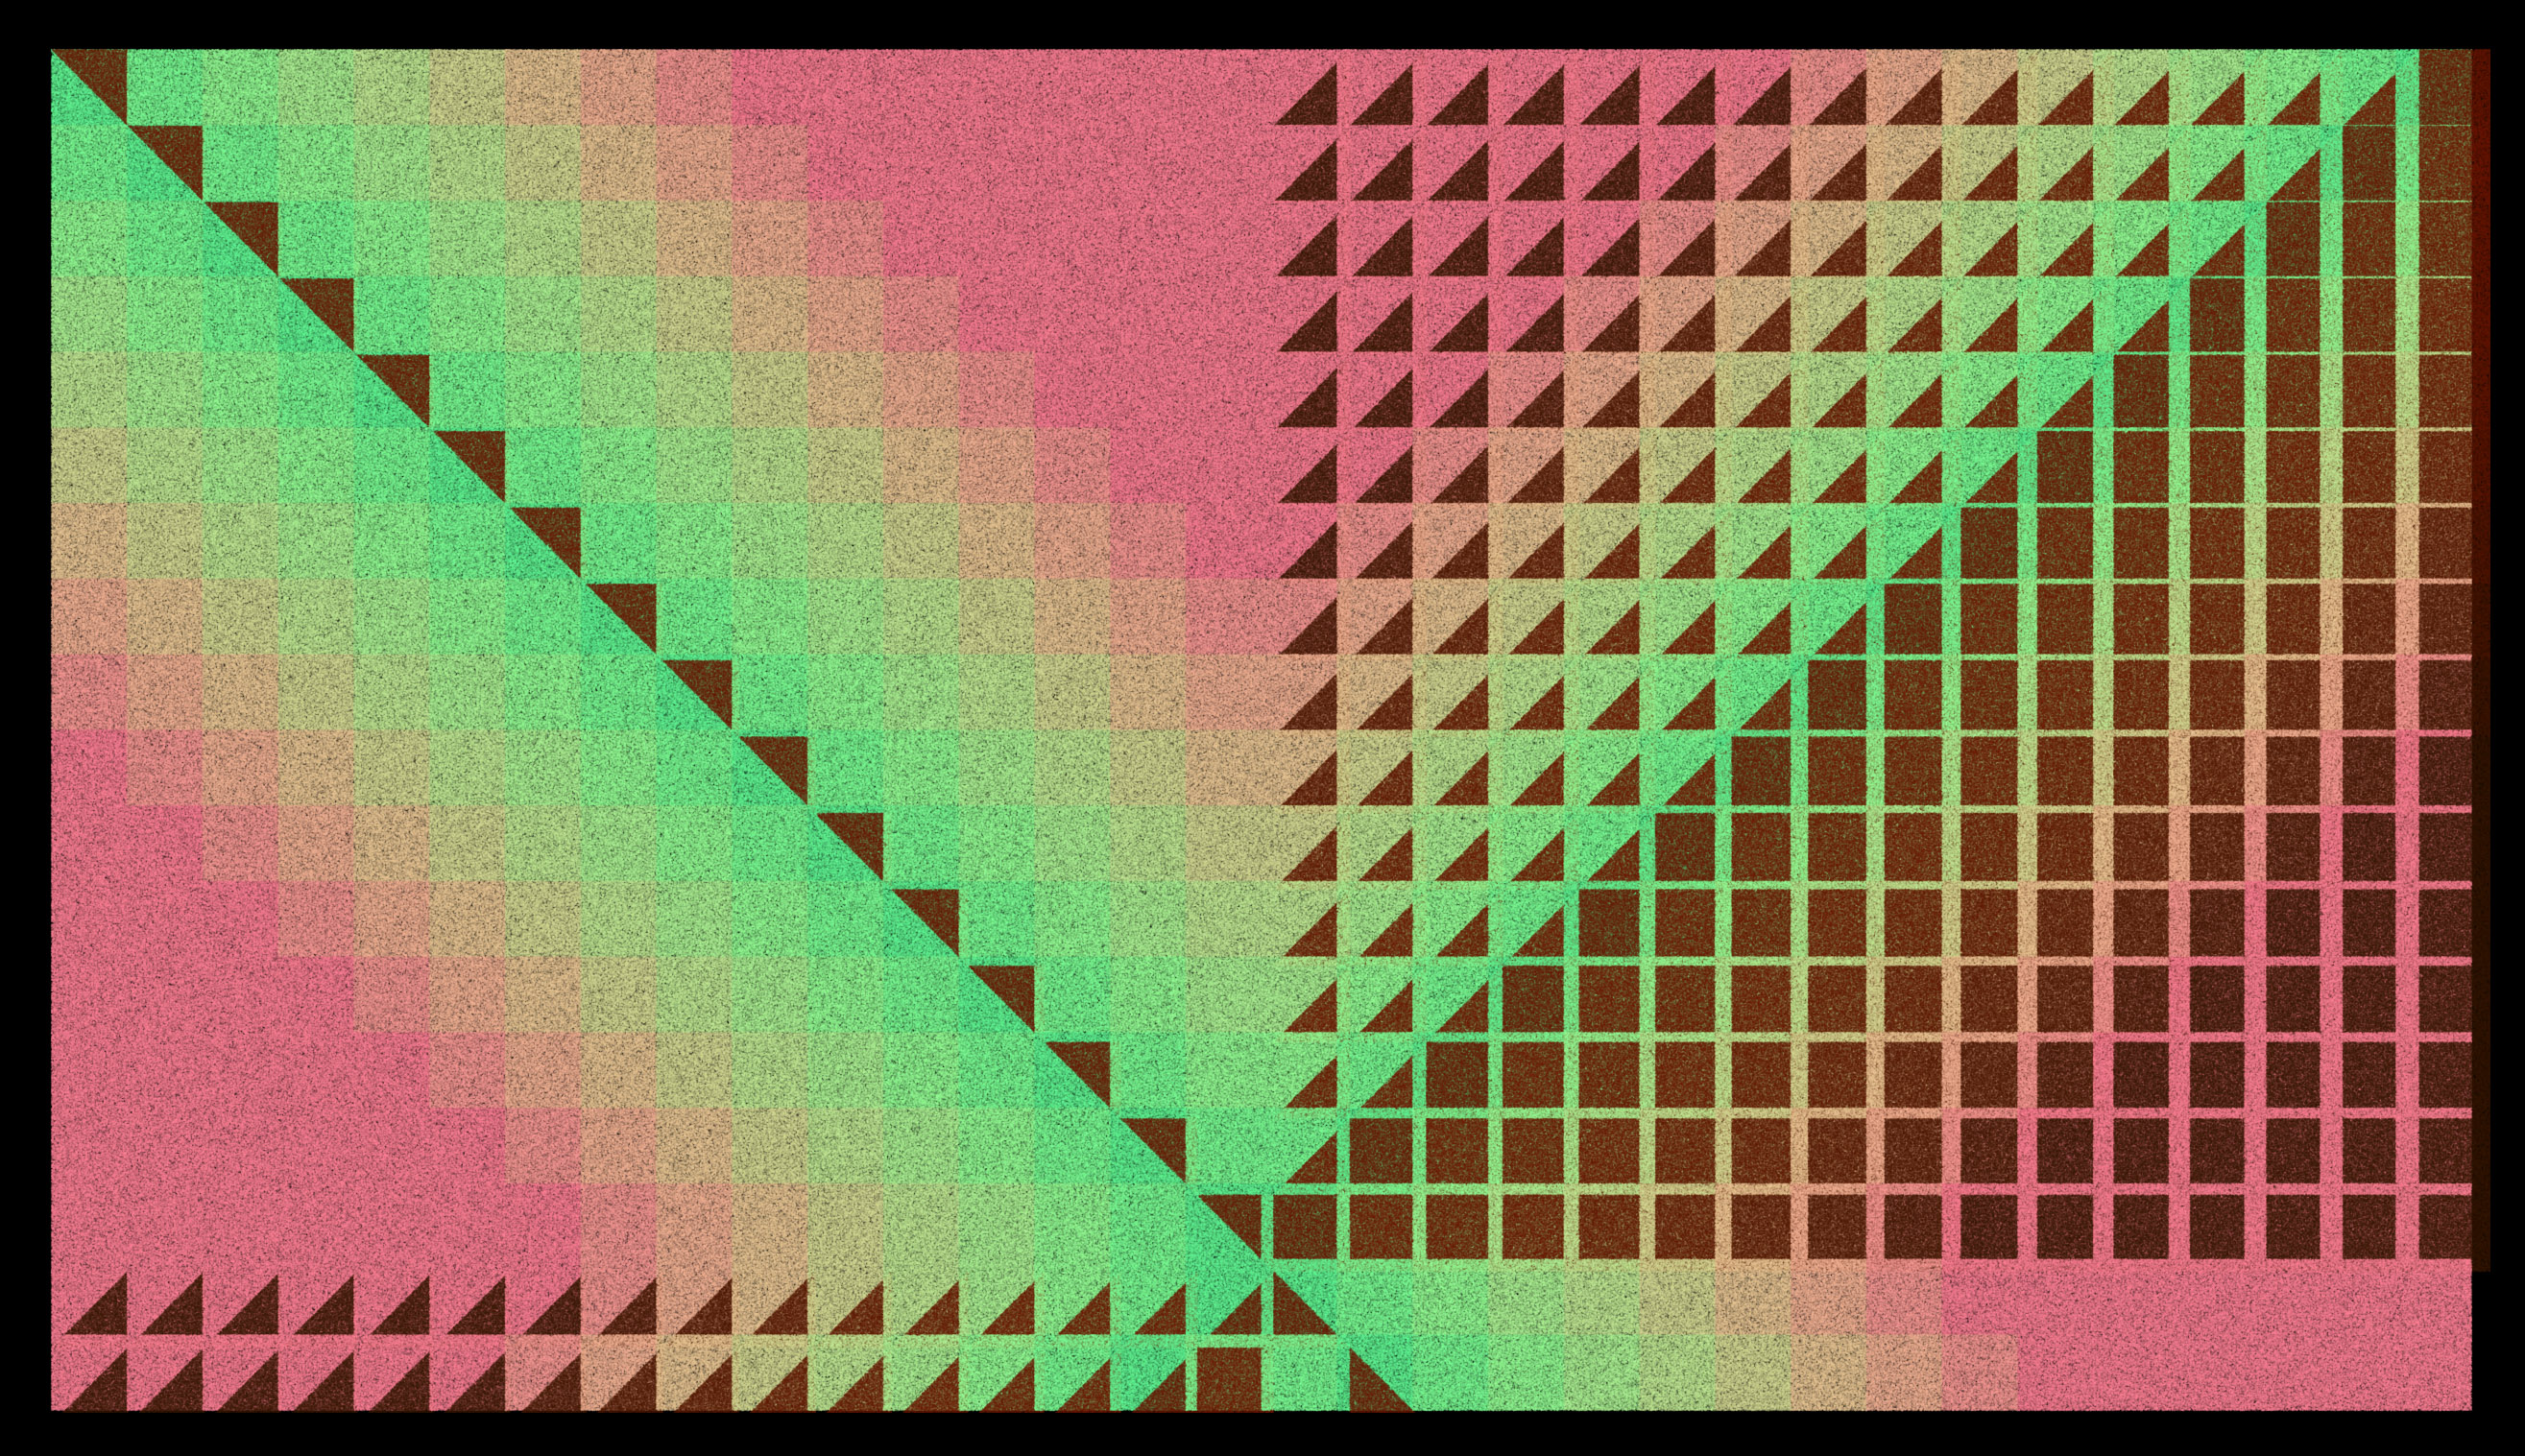
\includegraphics[width=1\textwidth]{images/pavage004.jpg}
\caption{Un exemple du troisième algorithme de coloration des tuiles}
\label{thirdcoloralgorithm}
\end{figure}
